\documentclass{article}

\usepackage[a4paper]{geometry}

\usepackage{booktabs}
\usepackage{graphicx}
\usepackage{mathtools}
\usepackage{tabularx}

\title{Reward Inequality for Different Tailstorm Incentive Schemes}
\author{Patrik Keller}

\begin{document}

\maketitle

\section{Tailstorm}

\paragraph{Global data structure}

Each block requires a proof-of-work. Each block $b$ has two integer properties 
\begin{enumerate}
\item integer $\operatorname{depth}(b)$
\item integer $\operatorname{epoch}(b)$
\end{enumerate}

There are two kind of blocks. Each sub block $b'$ references exactly one block $b$. For sub blocks it holds that
$\operatorname{depth}(b') = \operatorname{depth}(b) + 1$ and $\operatorname{epoch}(b') = \operatorname{epoch}(b)$.

A strong block $b$ references a list $l$ of blocks all having the same epoch $e$. Let $Q$ denote the set of sub blocks with epoch $e$ that are member of $l$ or in the history of a member of $l$. If $b$ is valid it holds that
\begin{enumerate}
  \item $|Q| = k - 1$
  \item $\operatorname{epoch}(b) = e + 1$
  \item $\operatorname{depth}(b) = 0$
\end{enumerate}

\paragraph{Protocol}

Nodes maintain a preferred block $b$. Whenever a node is activated, it attaches a new valid block to the global data structure. It first tries to attach a strong block that references $b$. If this is not possible, it attaches a sub block instead.

Whenever a node becomes aware of a new block $b'$ it updates it preference. A node prefers $b'$ over $b$ if $\operatorname{epoch}(b') > \operatorname{epoch}(b)$ or $\operatorname{epoch}(b') = \operatorname{epoch}(b) \wedge \operatorname{depth}(b') > \operatorname{depth}(b)$. In case of a tie, nodes prefer the block first received.

\section{Incentive Schemes}

All reward schemes have in common that rewards are only assigned to (sub-)blocks that end up in the common chain of all participating nodes.

\paragraph{block}
Constant reward per strong block.

\paragraph{constant}
Constant reward per sub and strong block.

\paragraph{discount}
The rewards for an epoch are discounted for the depth of the resulting epoch tree.

\paragraph{punish}
For any epoch tree, only the sub blocks on the longest path get a reward. The assigned rewards are constant.

\paragraph{hybrid}
A combination of discount and punish.

\section{Honest Network}

We simulate 10 honest nodes executing the protocol in a fully connected network with uniformly distributed propagation delays.
We label the nodes $1, 2, \dots, 10$. The nodes have compute powers $1, 2, \dots, 10$.
We simulate $1 000 000$ activations per combination of input parameters.
After protocol simulation we search for the longest common chain, i.\,e., the block with the biggest epoch number that is also in the history of all nodes.
We apply the incentive scheme to this longest common chain.

\paragraph{Efficiency of weakest miner}

Let $\operatorname{reward}(i)$ denote the rewards assigned to node $i$ and $\operatorname{activations}(i)$ the amount of activations it received during the simulation.
We define a node's efficiency as follows.
\[
  \operatorname{efficiency}(i) =
  \frac{
    \frac{\operatorname{reward}(i)}{\sum_{j=1}^{10}{\operatorname{reward}(j)}}
    }{
    \frac{\operatorname{activations}(i)}{\sum_{j=1}^{10}{\operatorname{activations}(j)}}
  }
\]

We call node $1$ the weakest miner.
Table~\ref{tab:efficiency_weakest} lists the efficiency of the weakest miner for different combinations of block interval and protocol parameter $k$ (rows) and incentive schemes (columns). We observe that efficiency of the weakest miner is consistently below 1. The incentive schemes \textbf{constant} and \textbf{discount} yield the more rewards for the weakest miner. Depending on $k$, the might be better of with the \textbf{block} incentive scheme or the \textbf{punish} and \textbf{hybrid} incentive schemes. The latter two yield comparable results for all combinations of block interval and $k$.

% TODO: Add orphan rate columns.

\begin{table}
  \caption{
    Efficiency of the weakest miner for different block intervals (row), k (row), and incentive schemes (column).
    An efficiency of one implies that the weakest miner's relative rewards equal its relative compute power.\strut
  }
  \label{tab:efficiency_weakest}
  \begin{tabular}{llrrrrr}
\toprule
      & Incentive Scheme &     block &  constant &  discount &    hybrid &    punish \\
Block Interval & k &           &           &           &           &           \\
\midrule
30.0  & 1   &  0.992089 &  0.992089 &  0.992089 &  0.992089 &  0.992089 \\
      & 2   &  0.979370 &  0.984524 &  0.984524 &  0.984524 &  0.984524 \\
      & 4   &  0.969144 &  0.982597 &  0.979192 &  0.968015 &  0.968317 \\
      & 8   &  0.945803 &  0.983121 &  0.977423 &  0.941657 &  0.943261 \\
      & 16  &  0.882500 &  0.985670 &  0.980514 &  0.879682 &  0.880920 \\
      & 32  &  0.792723 &  0.979461 &  0.974919 &  0.763680 &  0.763675 \\
      & 64  &  0.706071 &  0.978301 &  0.974315 &  0.556296 &  0.557793 \\
      & 128 &  0.346941 &  0.977279 &  0.973979 &  0.296788 &  0.297215 \\
60.0  & 1   &  0.997408 &  0.997408 &  0.997408 &  0.997408 &  0.997408 \\
      & 2   &  0.984510 &  0.992090 &  0.992090 &  0.992090 &  0.992090 \\
      & 4   &  0.982581 &  0.991625 &  0.989028 &  0.984381 &  0.985651 \\
      & 8   &  0.986718 &  0.990231 &  0.987405 &  0.969290 &  0.969853 \\
      & 16  &  0.915465 &  0.990583 &  0.987649 &  0.941182 &  0.941490 \\
      & 32  &  0.925923 &  0.991585 &  0.989370 &  0.876803 &  0.876778 \\
      & 64  &  0.755949 &  0.989245 &  0.986418 &  0.759216 &  0.760301 \\
      & 128 &  0.638507 &  0.988145 &  0.985370 &  0.548299 &  0.550002 \\
120.0 & 1   &  0.998914 &  0.998914 &  0.998914 &  0.998914 &  0.998914 \\
      & 2   &  1.014695 &  0.995182 &  0.995182 &  0.995182 &  0.995182 \\
      & 4   &  1.004402 &  0.996496 &  0.994990 &  0.991689 &  0.992175 \\
      & 8   &  1.013124 &  0.996954 &  0.996247 &  0.988202 &  0.987836 \\
      & 16  &  0.963169 &  0.995384 &  0.993471 &  0.966911 &  0.967085 \\
      & 32  &  0.950865 &  0.996880 &  0.994839 &  0.937554 &  0.937743 \\
      & 64  &  0.892522 &  0.994865 &  0.993553 &  0.878929 &  0.879094 \\
      & 128 &  0.761628 &  0.994631 &  0.993289 &  0.755009 &  0.754911 \\
300.0 & 1   &  0.999150 &  0.999150 &  0.999150 &  0.999150 &  0.999150 \\
      & 2   &  1.001489 &  0.998209 &  0.998209 &  0.998209 &  0.998209 \\
      & 4   &  0.988634 &  0.997473 &  0.997453 &  0.996140 &  0.995720 \\
      & 8   &  1.013500 &  0.999380 &  0.999127 &  0.996325 &  0.996137 \\
      & 16  &  1.004682 &  0.996407 &  0.995822 &  0.983355 &  0.983204 \\
      & 32  &  0.965302 &  0.998942 &  0.998272 &  0.979342 &  0.979332 \\
      & 64  &  0.983097 &  0.997505 &  0.997446 &  0.949199 &  0.948667 \\
      & 128 &  1.062957 &  0.999608 &  0.999635 &  0.904243 &  0.903759 \\
600.0 & 1   &  0.999739 &  0.999739 &  0.999739 &  0.999739 &  0.999739 \\
      & 2   &  1.009494 &  0.999407 &  0.999407 &  0.999407 &  0.999407 \\
      & 4   &  1.004113 &  0.999346 &  0.999459 &  0.998562 &  0.998153 \\
      & 8   &  1.011927 &  0.999362 &  0.998755 &  0.996917 &  0.997235 \\
      & 16  &  0.993903 &  0.999748 &  0.999647 &  0.994388 &  0.994160 \\
      & 32  &  0.954984 &  0.999276 &  0.999328 &  0.984063 &  0.983589 \\
      & 64  &  0.952486 &  0.998924 &  0.998324 &  0.970315 &  0.970486 \\
      & 128 &  0.870018 &  0.998832 &  0.998715 &  0.948818 &  0.948775 \\
\bottomrule
\end{tabular}

\end{table}

\paragraph{Gini Inequality}

Similar to above.
Instead of looking at the efficiency of a single miner, we now look at the inequality of rewards between all nodes.
We use the Gini coefficient as a measure for inequality.
The inequality between the compute powers is 0.3.
Values lower than 0.3 would speak for reduced inequality.
However, as we observe in Table~\ref{tab:reward_gini}, rewards inhibit higher inequality for all combinations of $k$, block interval, and incentive scheme.

\begin{table}
  \caption{
    Gini coefficient of rewards for different block intervals (row), $k$ (row), and incentive schemes (column).
    Lower values stand for less inequality. The Gini coefficient of compute power is $0.3$.\strut
  }
  \label{tab:reward_gini}
  \begin{tabular}{llrrrrr}
\toprule
      & Incentive Scheme &     block &  constant &  discount &    hybrid &    punish \\
Block Interval & k &           &           &           &           &           \\
\midrule
30.0  & 1   &  0.301341 &  0.301341 &  0.301341 &  0.301341 &  0.301341 \\
      & 2   &  0.303348 &  0.302833 &  0.302833 &  0.302833 &  0.302833 \\
      & 4   &  0.305474 &  0.303605 &  0.304212 &  0.305758 &  0.305595 \\
      & 8   &  0.310609 &  0.303909 &  0.304887 &  0.311687 &  0.311513 \\
      & 16  &  0.323702 &  0.303854 &  0.304898 &  0.323519 &  0.323269 \\
      & 32  &  0.343210 &  0.304800 &  0.305874 &  0.349275 &  0.348806 \\
      & 64  &  0.377924 &  0.305462 &  0.306460 &  0.398329 &  0.397588 \\
      & 128 &  0.444700 &  0.307160 &  0.308140 &  0.478010 &  0.476899 \\
60.0  & 1   &  0.300484 &  0.300484 &  0.300484 &  0.300484 &  0.300484 \\
      & 2   &  0.301437 &  0.301341 &  0.301341 &  0.301341 &  0.301341 \\
      & 4   &  0.302621 &  0.302038 &  0.302462 &  0.303290 &  0.303116 \\
      & 8   &  0.306823 &  0.302334 &  0.302835 &  0.306213 &  0.306142 \\
      & 16  &  0.314684 &  0.302272 &  0.302875 &  0.312181 &  0.312095 \\
      & 32  &  0.323930 &  0.301933 &  0.302513 &  0.324570 &  0.324422 \\
      & 64  &  0.344082 &  0.302635 &  0.303163 &  0.350253 &  0.350017 \\
      & 128 &  0.379089 &  0.302045 &  0.302583 &  0.397107 &  0.396721 \\
120.0 & 1   &  0.300198 &  0.300198 &  0.300198 &  0.300198 &  0.300198 \\
      & 2   &  0.301106 &  0.301277 &  0.301277 &  0.301277 &  0.301277 \\
      & 4   &  0.301921 &  0.301307 &  0.301461 &  0.301842 &  0.301811 \\
      & 8   &  0.303194 &  0.301422 &  0.301693 &  0.303501 &  0.303474 \\
      & 16  &  0.305443 &  0.301034 &  0.301311 &  0.305951 &  0.305940 \\
      & 32  &  0.312274 &  0.301169 &  0.301473 &  0.312458 &  0.312438 \\
      & 64  &  0.318006 &  0.300720 &  0.301017 &  0.324140 &  0.324098 \\
      & 128 &  0.335267 &  0.300659 &  0.300984 &  0.349340 &  0.349235 \\
300.0 & 1   &  0.299957 &  0.299957 &  0.299957 &  0.299957 &  0.299957 \\
      & 2   &  0.300812 &  0.300929 &  0.300929 &  0.300929 &  0.300929 \\
      & 4   &  0.301003 &  0.300958 &  0.301013 &  0.301146 &  0.301136 \\
      & 8   &  0.300130 &  0.300952 &  0.301071 &  0.301801 &  0.301784 \\
      & 16  &  0.300827 &  0.300614 &  0.300761 &  0.302722 &  0.302694 \\
      & 32  &  0.304996 &  0.299946 &  0.300086 &  0.304106 &  0.304096 \\
      & 64  &  0.308948 &  0.300634 &  0.300764 &  0.310106 &  0.310098 \\
      & 128 &  0.325061 &  0.300556 &  0.300657 &  0.319847 &  0.319845 \\
600.0 & 1   &  0.299879 &  0.299879 &  0.299879 &  0.299879 &  0.299879 \\
      & 2   &  0.300703 &  0.300752 &  0.300752 &  0.300752 &  0.300752 \\
      & 4   &  0.300425 &  0.300764 &  0.300815 &  0.300915 &  0.300897 \\
      & 8   &  0.299081 &  0.300844 &  0.300920 &  0.301272 &  0.301246 \\
      & 16  &  0.303110 &  0.300669 &  0.300740 &  0.301634 &  0.301620 \\
      & 32  &  0.308286 &  0.300017 &  0.300099 &  0.302392 &  0.302376 \\
      & 64  &  0.312363 &  0.300627 &  0.300710 &  0.305128 &  0.305107 \\
      & 128 &  0.303825 &  0.299617 &  0.299678 &  0.308789 &  0.308790 \\
\bottomrule
\end{tabular}

\end{table}

\section{Withholding Attacks}

We simulate two nodes in a network with zero delays.
Node $a$ implements a withholding strategy.
We call this node attacker.
Node $b$ acts honestly, i.\,e, follows the protocol as specified.
We call this node defender.

We assign compute $\alpha$ to the attacker and $1-\alpha$ to the defender.

\subsection{Strategies}

\paragraph{Common to All Strategies}
The attacker maintains a private fork of the chain and releases blocks tactically.
If the private chain falls behind the public chain, i.\,e., an honest node would prefer the public chain over the withheld private chain, the attacker adopts the private chain.

\paragraph{Release Strong Block}
The attacker withholds all sub blocks until he can form a strong block.
He then releases this strong block together with all referenced sub blocks.
When forming a strong block, the attacker prefers his own sub blocks in order to maximize his own rewards.

\paragraph{Override Block}
The attacker withholds all blocks (sub and strong) until the defender forms a strong block.
He then releases a withheld strong block including all referenced sub blocks as well as one sub block that confirms the just released strong block.
The goal is to override the most recent defender strong block.

\paragraph{Override Catch-Up}
The attacker withholds all blocks (sub and strong) as long the withheld chain is clearly better than the defender's chain.
When the attacker is about to catch up, i.\,e., needs only one more puzzle solution to match the defender's chain, the attacker releases his private chain.
The goal is to override all defender blocks since the attacker started to withhold blocks.

\subsection{Measurements}

We measure the attacker's reward dependent on $k$, $\alpha$, the strategy, and the reward scheme.

We simulate $1 000 000$ activations per combination of input parameters.
After protocol simulation we search for the longest common chain, i.\,e., the block with the biggest epoch number that is also in the history of all nodes.
We apply the incentive scheme to this longest common chain.

Figure~\ref{fig:withholding_absolute} shows the attacker's rewards per time. The unit of time is 1. The activation delay is one puzzle solution per 1 unit of time. We observe that in the short run, i.\,e.\ before difficulty adjustment, all dishonest strategies reduce the attackers rewards.

We observe confirmed blocks per simulated time and then rescale the simulation time by this factor.
This emulates the effect of a difficulty adjustment algorithm.%
\footnote{In real world settings, the difficulty affects the orphan rate. Here we have zero network delays, and orphan rate does not depend on the difficulty.}
Figure~\ref{fig:withholding_daa} shows the attacker's rewards per time \emph{after} difficulty adjustment.
The unit of time is rescaled such that we observe one confirmed puzzle solution per 1 unit of time.
We observe that in the long run certain strategies benefit the attacker.
However, the \textbf{discount} incentive scheme dampens the profitability of the attack.

Figure~\ref{fig:withholding_relative} shows the attacker's rewards relative to the overall rewards assigned.
This is a measure used in selfish mining to model long term rewards after difficulty adjustment.
We observe that the positive effect of the \textbf{discount} incentive scheme is mostly hidden by this metric.

\begin{figure}
  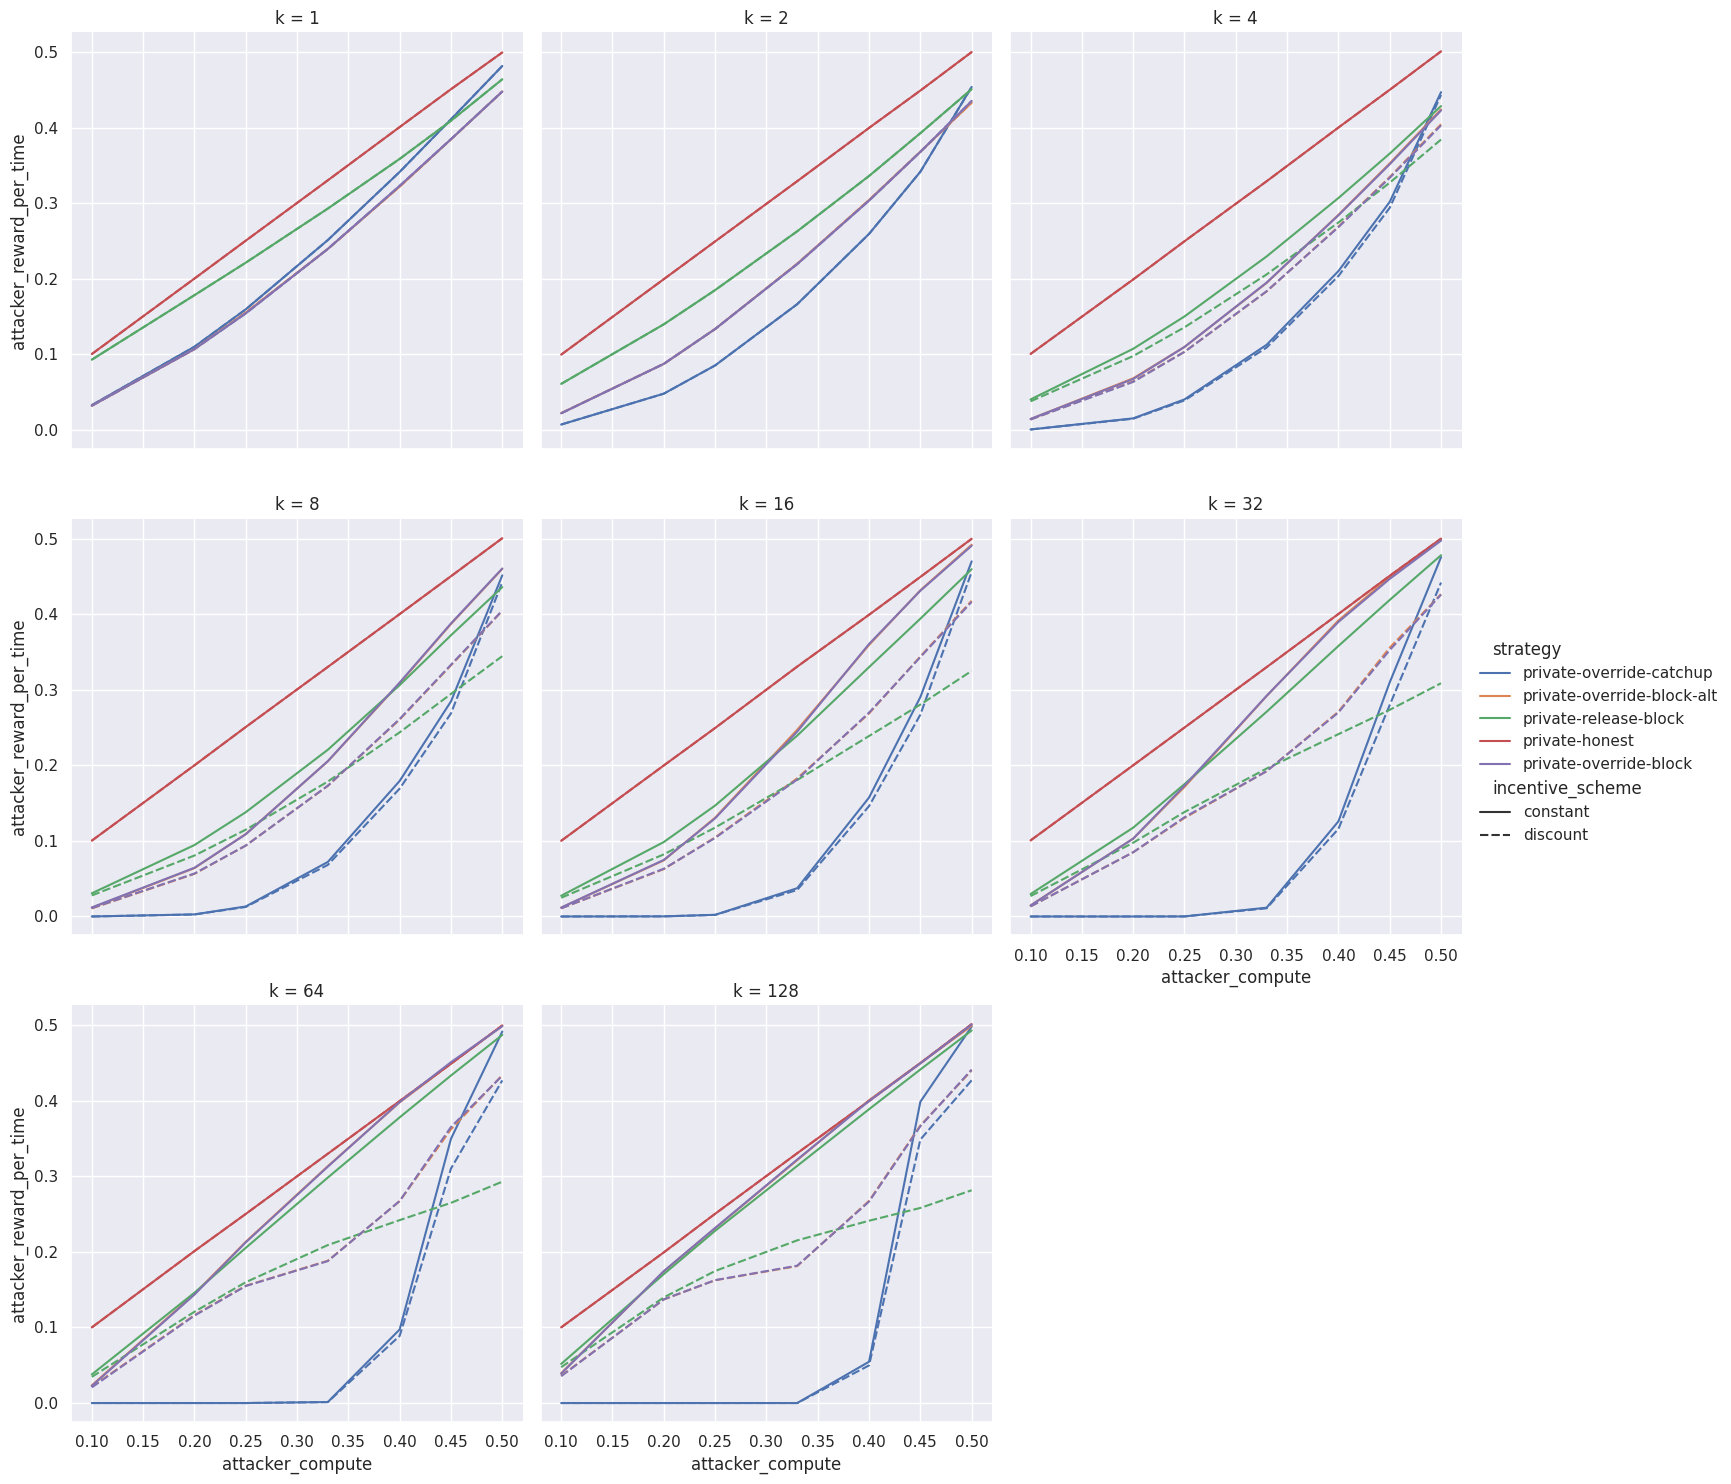
\includegraphics[width=\linewidth]{fig/withholding_absolute}
  \caption{
    The attacker's absolute reward (per time) depends on $k$, $\alpha$, the withholding strategy, and the reward scheme.
  }
  \label{fig:withholding_absolute}
\end{figure}

\begin{figure}
  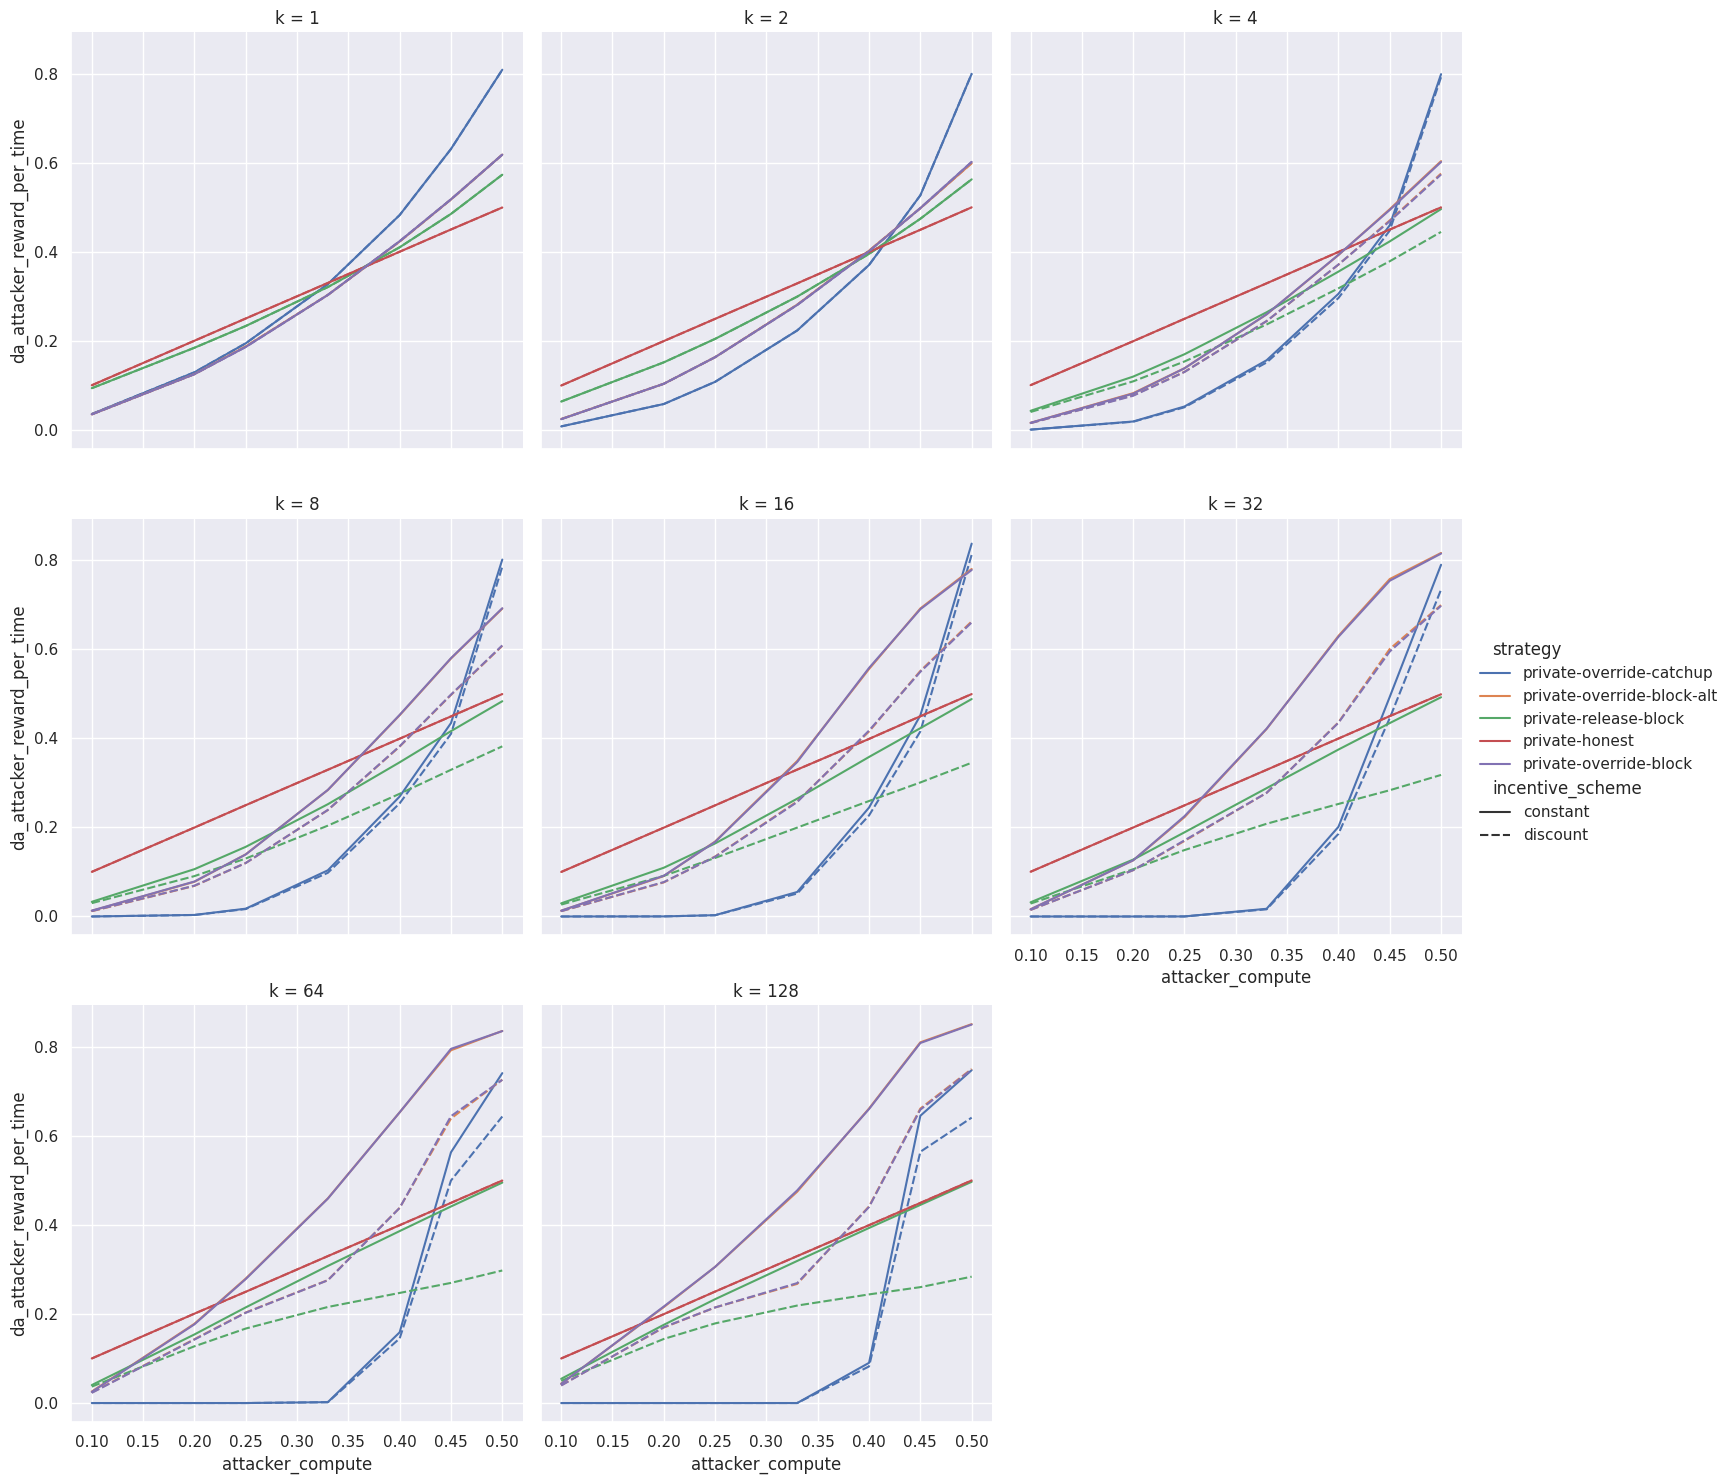
\includegraphics[width=\linewidth]{fig/withholding_daa}
  \caption{
    The attacker's absolute reward (per time) after difficulty adjustment depends on $k$, $\alpha$, the withholding strategy, and the reward scheme.
  }
  \label{fig:withholding_daa}
\end{figure}

\begin{figure}
  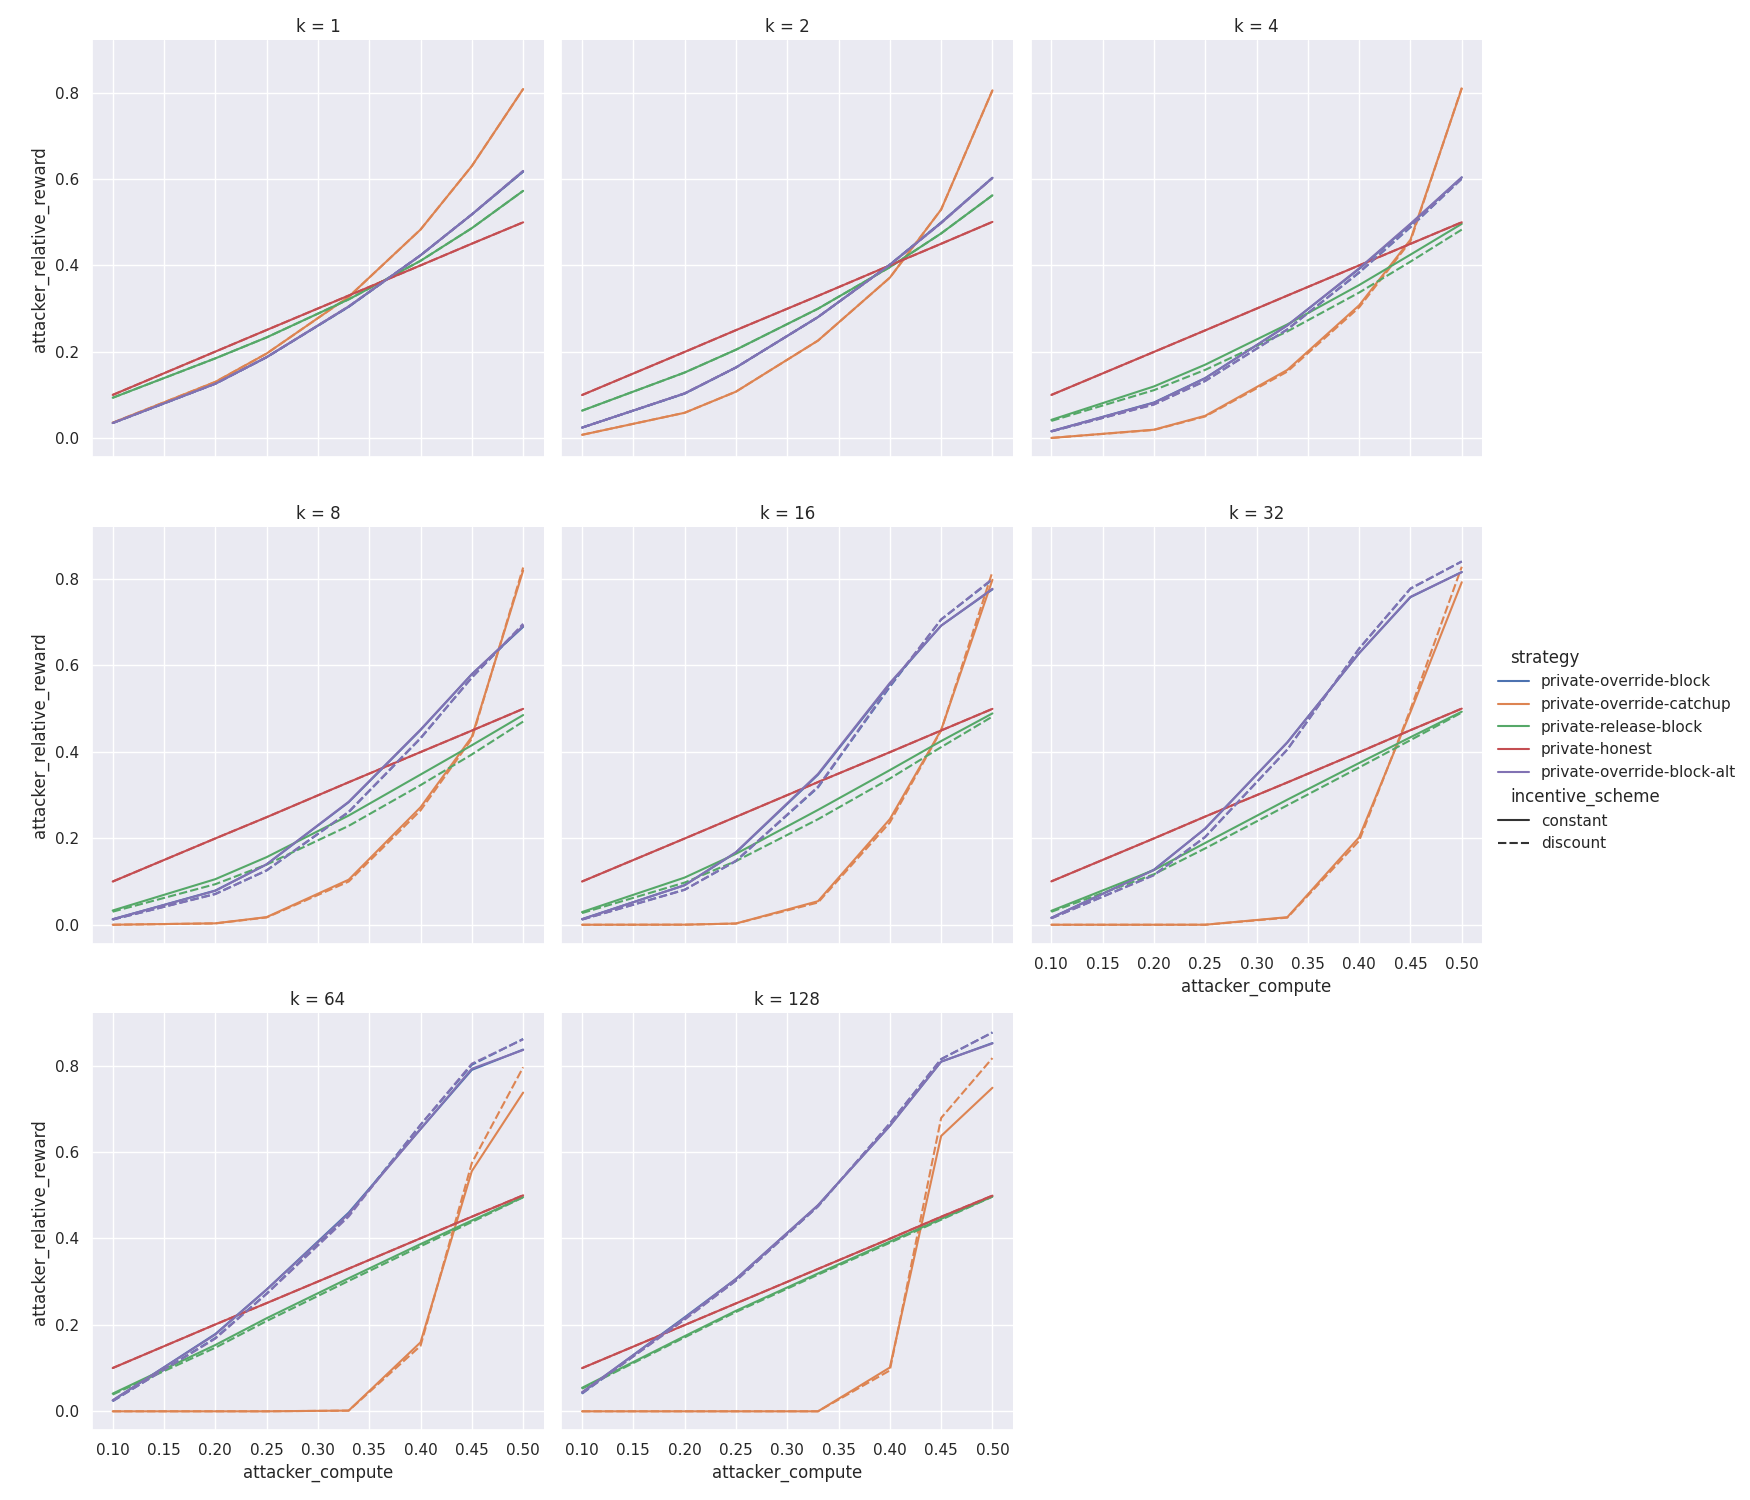
\includegraphics[width=\linewidth]{fig/withholding_relative}
  \caption{
    The attacker's relative share of reward depends on $k$, $\alpha$, the withholding strategy, and the reward scheme.
  }
  \label{fig:withholding_relative}
\end{figure}

\end{document}
